% !Mode:: "TeX:ACP:Hard"
\documentclass[14pt,hyperref={CJKbookmarks=true}]{beamer}

%\usepackage[space,noindent]{ctex}
\usepackage{mathrsfs}
\usepackage{amsfonts,amssymb}
\usepackage{amsmath}
\usepackage{graphicx}
\usepackage{subcaption}
\usepackage{lmodern}
\usepackage[labelformat=empty,font=scriptsize,skip=0pt,justification=centering,singlelinecheck=false]{caption}
\usepackage{bibentry}
\usepackage{csquotes}
\usepackage{amsthm}
\usepackage{color}
\theoremstyle{plain}
\usepackage{booktabs}
\newtheorem{thm}{Theorem}[section]
\newtheorem{lem}[thm]{Lemma}
\newtheorem{prop}[thm]{Proposition}
\newtheorem*{cor}{Corollary}

\theoremstyle{definition}
\newtheorem{defn}{Definition}[section]
\newtheorem{conj}{Conjecture}[section]
\newtheorem{exmp}{Example}[section]

\theoremstyle{remark}
\newtheorem*{rem}{Remark}

%\captionsetup{font={scriptsize}}
\captionsetup[figure]{name=Fig., labelsep=space}
%remove the icon
\setbeamertemplate{bibliography item}{}
%remove line breaks
\setbeamertemplate{bibliography entry title}{}
\setbeamertemplate{bibliography entry location}{}
\setbeamertemplate{bibliography entry note}{}
\usetheme{AnnArbor}
%\usetheme{CambridgeUS}
%\usetheme{Berlin}
%\usetheme{Dresden}
%\usecolortheme{beaver}
%\setbeamercolor{itemize item}{fg=black!80!black}
\usefonttheme{serif}     % Font theme: serif
\usepackage{ccfonts}     % Font family: Concrete Math
\usepackage[T1]{fontenc} % Font encoding: T1
\setbeamercolor{normal text}{bg=black!10}
\setbeamerfont{caption}{size=\tiny}
\graphicspath{{./image/}}

\begin{document}

%\section{Title}


\title[IACAS]{Filter and its Applications}
%\subtitle[副题简称]{论文副题}
\author{Tian Chen}
\institute[]{Institute of Automation, Chinese Academy of Sciences\\University of Chinese Academy of Sciences}
\date[]{2017.05.13}


\begin{frame}
\titlepage
\end{frame}


%% Outline page


\begin{frame}
\frametitle{Quick Overview} 
\small\tableofcontents
\end{frame}

%% 
\section{Introduction}
\frame{\tableofcontents[currentsection]}
\begin{frame}
\frametitle{Introduction} 
\begin{table}
\small
%\caption{Classification of System}
\begin{tabular}{c c c }
\toprule[1pt]
process & Linear Gaussian &Nonline Gaussian\\
\midrule[0.5pt]
motion model &$\mathbf{A}_{k}\mathbf{x}_{k-1}+\mathbf{B}_{k}\mathbf{u}_{k}+\mathbf{q}_{k}$ & $\mathbf{f}(\mathbf{x}_{k-1},\mathbf{u}_{k},\mathbf{q}_{k})$\\
observation model &  $\mathbf{H}_k\mathbf{x}_k+\mathbf{r}_k$ &  $\mathbf{g}(\mathbf{x}_k,\mathbf{r}_k)$ \\
Estimation & kalman Filter& EKF, particle Filter\\
\bottomrule[1pt]
\end{tabular}
\end{table}
\begin{figure}
\centering
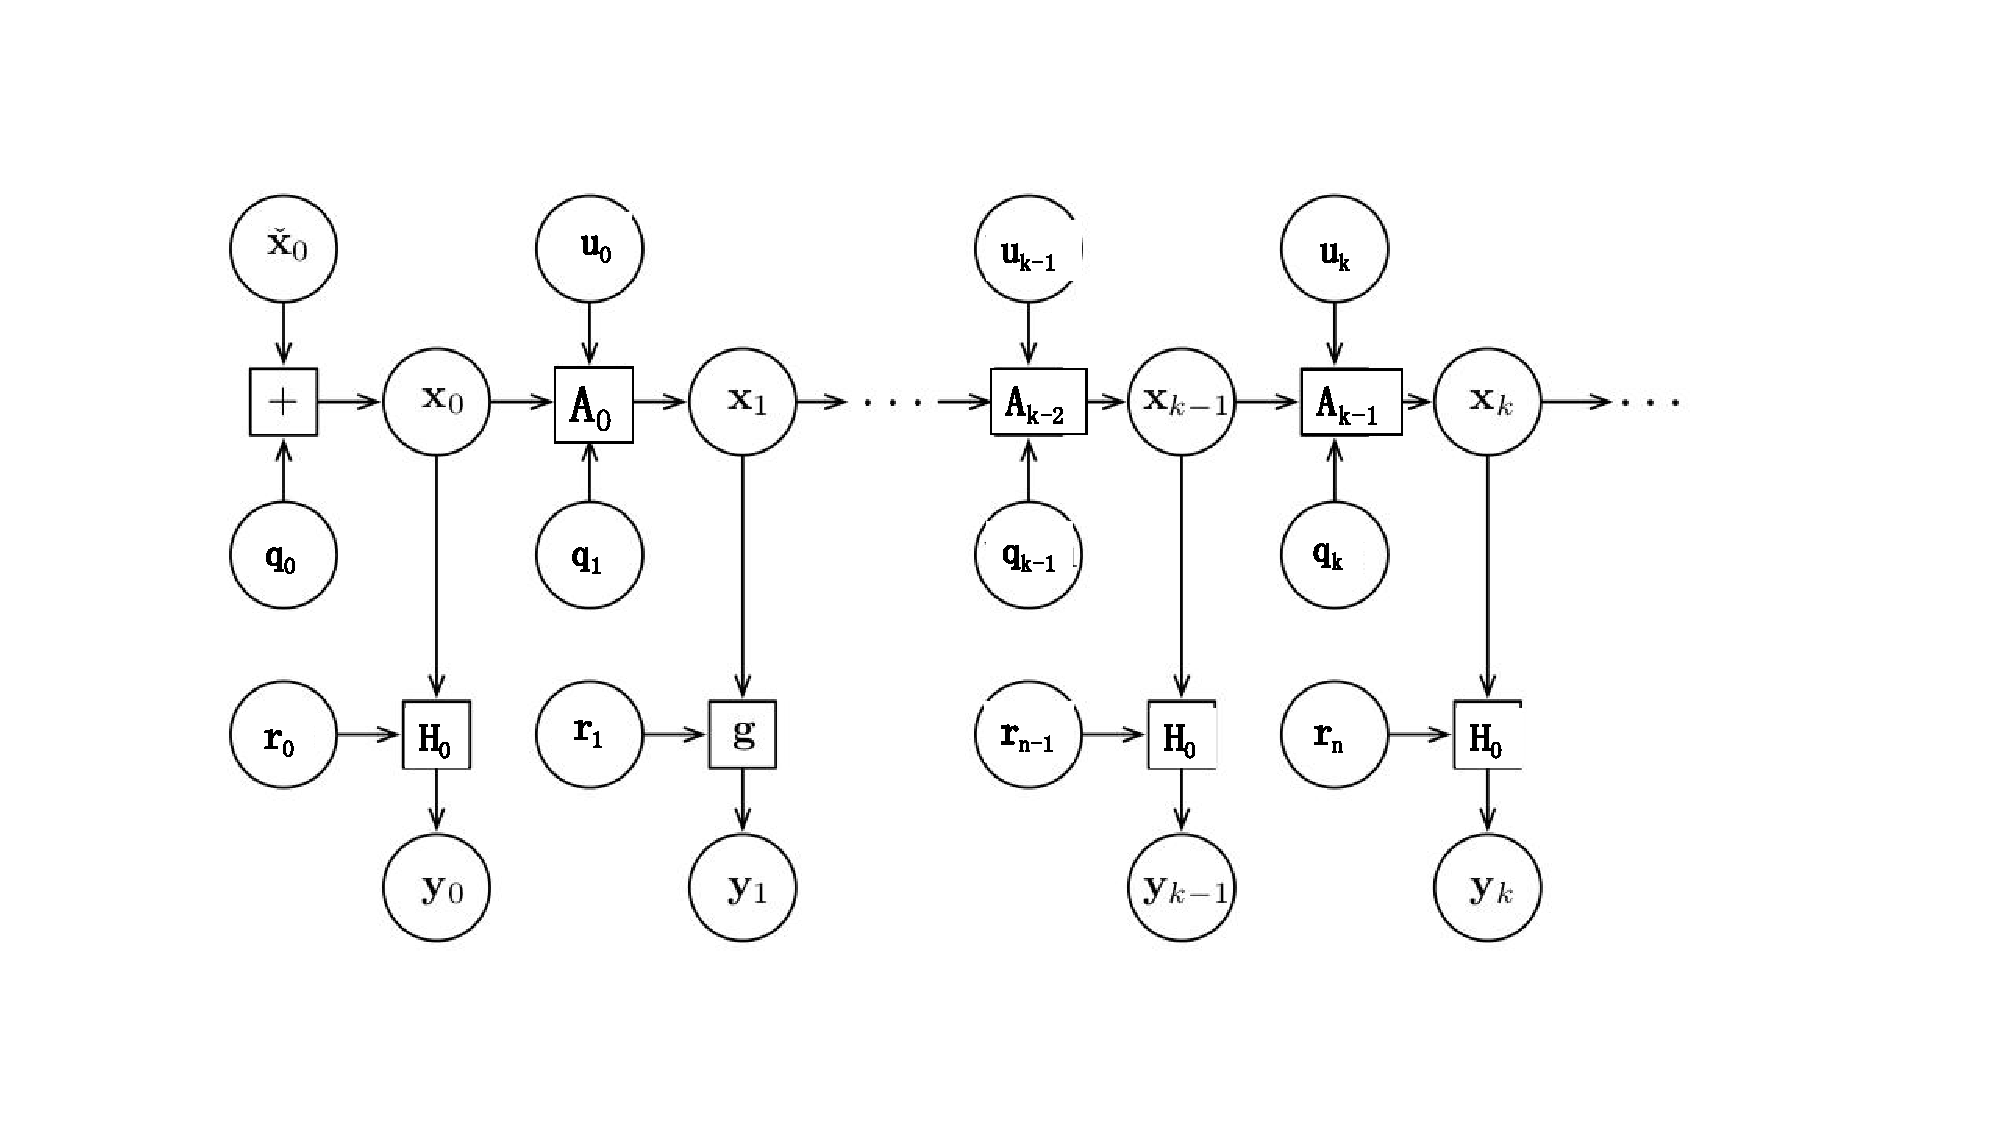
\includegraphics[width=0.45\linewidth]{state1.pdf}
\quad
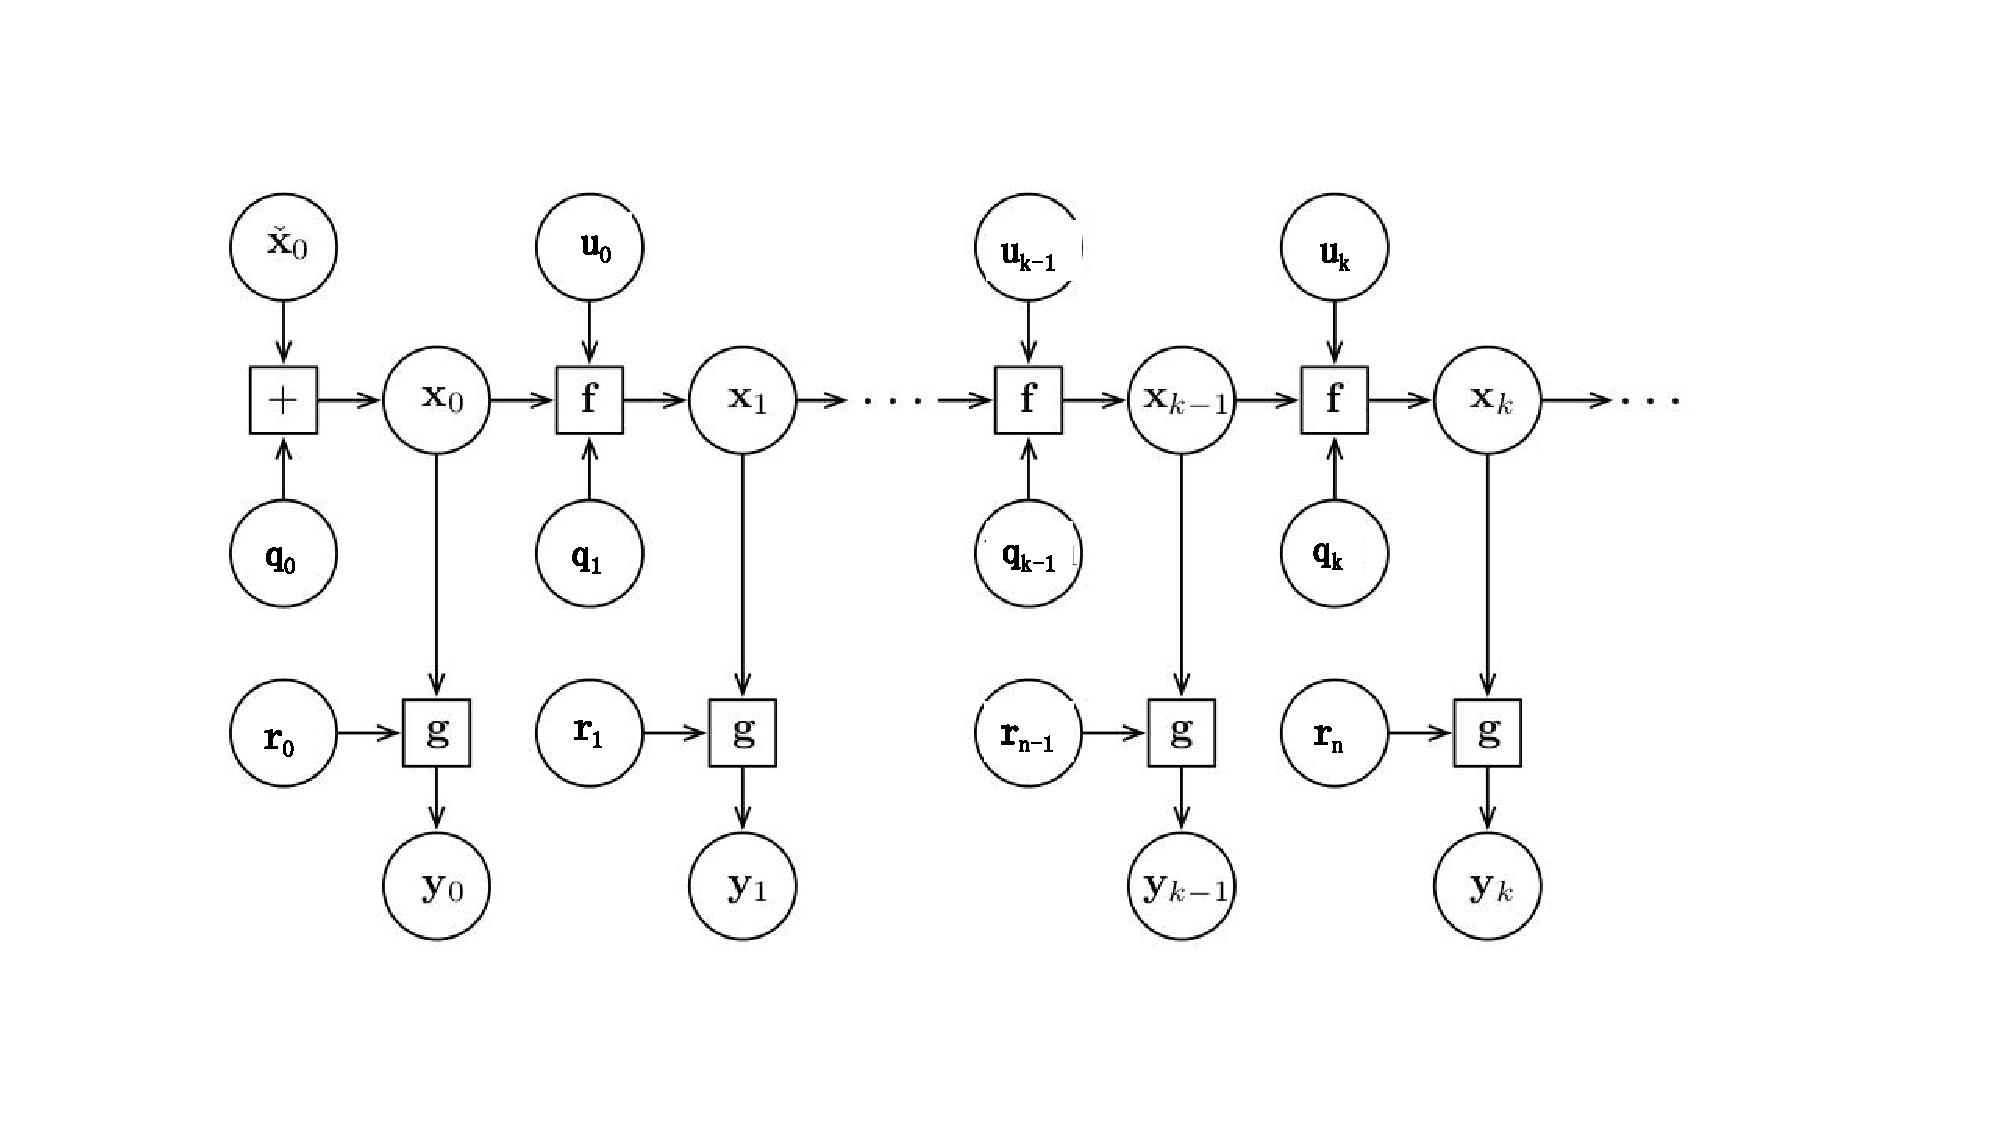
\includegraphics[width=0.45\linewidth]{state2.pdf}
\end{figure}

\end{frame}


\section{Filter}
\frame{\tableofcontents[currentsection]}
\subsection{Linear Gaussian Process}
\begin{frame}
\frametitle{State Space Model} 
\small
%\begin{block}{State Space Model}
\begin{equation}
\begin{cases}
\mathbf{x}_k=\mathbf{A}_{k}\mathbf{x}_{k-1}+\mathbf{B}_{k}\mathbf{u}_{k}+\mathbf{q}_{k}\\
\mathbf{y}_k=\mathbf{H}_k\mathbf{x}_k+\mathbf{r}_k
\end{cases} 
\end{equation}
%\end{block}
\pause
\begin{equation*}
\begin{split}
\text{system state:}\quad&\mathbf{x}_k\in\mathbb{R}^N\\
\text{input state:}\quad &\mathbf{u}_k\in\mathbb{R}^N\\
\text{process noise:}\quad &\mathbf{q}_k\in\mathbb{R}^N\sim \mathcal{N}(\mathbf{0},\mathbf{Q}_0)\\
\text{measurement:}\quad& \mathbf{y}_k\in\mathbb{R}^M\\
\text{measurement noise:}\quad& \mathbf{r}_k\in\mathbb{R}^M\sim \mathcal{N}(\mathbf{0},\mathbf{R}_0)\\
\end{split}
\end{equation*}
\end{frame}


\begin{frame}
\frametitle{State Space Model} 
\small
%\begin{block}{State Space Model}
\begin{equation}
\begin{cases}
\mathbf{x}_k=\mathbf{A}_{k}\mathbf{x}_{k-1}+\mathbf{B}_{k}\mathbf{u}_{k}+\mathbf{q}_{k}\\
\mathbf{y}_k=\mathbf{H}_k\mathbf{x}_k+\mathbf{r}_k
\end{cases} 
\end{equation}
%\end{block}
\pause
\begin{equation*}
\begin{split}
\text{transition matrix:}\quad& \mathbf{A}_k\in\mathbb{R}^{N\times N}\\
\text{control-input matrix:}\quad& \mathbf{B}_k\in\mathbb{R}^{N\times N}\\
\text{observation matrix:}\quad& \mathbf{H}_k\in\mathbb{R}^{M\times N}\\
\end{split}
\end{equation*}
\end{frame}

\begin{frame}
\frametitle{Kalman Filter} 
\small
{\bf{Predict}}
\begin{equation*}
\begin{split}
\text{Predicted state estimate} \quad \hat{\mathbf{x}}_{k\mid k-1} &= \mathbf{A}_k\hat{\mathbf{x}}_{k-1\mid k-1} + \mathbf{B}_k \mathbf{u}_k +\mathbf{q}_{k}\\
\text{Predicted estimate covariance} \quad\mathbf{P}_{k\mid k-1} &=  \mathbf{A}_k \mathbf{P}_{k-1\mid k-1} \mathbf{A}_k^\mathrm{T} + \mathbf{Q}_k\\
\text{measurement residual}\quad \tilde{\mathbf{y}}_k &= \mathbf{z}_k - \mathbf{H}_k\hat{\mathbf{x}}_{k\mid k-1}\\
\end{split}
\end{equation*}
\pause
{\bf{Update}}
\begin{equation*}
\begin{split}
\text{residual covariance}\quad\mathbf{S}_k& = \mathbf{H}_k \mathbf{P}_{k\mid k-1} \mathbf{H}_k^\mathrm{T} + \mathbf{R}_k \\
\text{ ''Optimal'' Kalman gain }\quad \mathbf{K}_k &= \mathbf{P}_{k\mid k-1}\mathbf{H}_k^\mathrm{T} \mathbf{S}_k^{-1}\\
\text{Updated state estimate}\quad \hat{\mathbf{x}}_{k\mid k} &= \hat{\mathbf{x}}_{k\mid k-1} + \mathbf{K}_k\tilde{\mathbf{y}}_k\\
\text{Updated estimate covariance}\quad\mathbf{P}_{k|k} &= (\mathbf{I} - \mathbf{K}_k \mathbf{H}_k) \mathbf{P}_{k|k-1} \\
\end{split}
\end{equation*}
\end{frame}

\begin{frame}
\small
\frametitle{R. E. Kalman}
\small
%\begin{block}{R.E.Kalman(1930-2016)}
%%%%%%%%figure of kalman
\begin{figure}
\centering
\begin{minipage}[t]{0.3\textwidth}
\centering
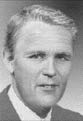
\includegraphics[width=2cm,height=3cm]{kalman0.jpg}
\end{minipage}
\begin{minipage}[t]{0.3\textwidth}
\centering
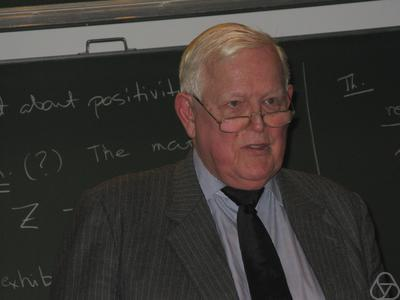
\includegraphics[width=4cm,height=3cm]{kalman.jpg}
\end{minipage}
\caption{\\Born 1930 in Hungry\\
Studied at MIT/Columbia\\
Developed filter in 1960/61}
\label{fig:graph}
\end{figure}
%%%%%%%%
\begin{displayquote}
His passing not only brought about personal loss but also a sad  reminder of the passing of a golden era in systems and control.
\end{displayquote}

%\begin{block}{Rudolf Kalman of Kalman Filter fame passed away yesterday}
%His passing not only brought about personal loss but also a sad  reminder of the passing of a golden era in systems and control.
%\end{block}
\end{frame}


\subsection{Nonlinear Gaussian Process}
\begin{frame}

\frametitle{Nonlinear Gaussian Process} 
\small
%\begin{block}{State Space Model}
\begin{equation}
\begin{cases}
\mathbf{x}_k=\mathbf{f}(\mathbf{x}_{k-1},\mathbf{u}_{k},\mathbf{q}_{k})\\
\mathbf{y}_k=\mathbf{g}(\mathbf{x}_k,\mathbf{r}_k)
\end{cases} 
\end{equation}
%\end{block}
%\pause
\begin{equation*}
\begin{split}
\text{transition model:}\quad& \mathbf{f}\\
\text{observation model:}\quad& \mathbf{g}\\
\end{split}
\end{equation*}
\pause
\begin{equation}
\begin{split}
\mathbf{f}(\mathbf{x}_{k-1},\mathbf{u}_{k},\mathbf{q}_{k})&\approx\check{\mathbf{x}}_k+\mathbf{A}_{k-1}(\mathbf{x}_{k-1}-\check{\mathbf{x}}_{k-1})+\mathbf{q}'_k\\
\mathbf{g}(\mathbf{x}_{k},\mathbf{u}_{k},\mathbf{r}_{k})&\approx\check{\mathbf{y}}_k+\mathbf{H}_{k}(\mathbf{x}_{k}-\check{\mathbf{x}}_{k})+\mathbf{r}'_k
\end{split}
\end{equation}
\end{frame}

\begin{frame}
\small
\frametitle{Extended Kalman Filter}{}
\small
{\bf{Predict}}
\begin{equation*}
\begin{split}
\text{Predicted state estimate} \quad \hat{\mathbf{x}}_{k\mid k-1} &= \mathbf{f}(\mathbf{x}_{k-1},\mathbf{u}_{k},\mathbf{q}_{k})\\
\text{Predicted estimate covariance} \quad\mathbf{P}_{k\mid k-1} &=  \mathbf{A}_k \mathbf{P}_{k-1\mid k-1} \mathbf{A}_k^\mathrm{T} + \mathbf{Q}'_k\\
\text{measurement residual}\quad \tilde{\mathbf{y}}_k &= \mathbf{z}_k - \mathbf{g}(\mathbf{x}_k,\mathbf{r}_k)\\
\end{split}
\end{equation*}
\pause
{\bf{Update}}
\begin{equation*}
\begin{split}
\text{residual covariance}\quad\mathbf{S}_k& = \mathbf{H}_k \mathbf{P}_{k\mid k-1} \mathbf{H}_k^\mathrm{T} + \mathbf{R}_k \\
\text{ ''Optimal'' Kalman gain }\quad \mathbf{K}_k &= \mathbf{P}_{k\mid k-1}\mathbf{H}_k^\mathrm{T} \mathbf{S}_k^{-1}\\
\text{Updated state estimate}\quad \hat{\mathbf{x}}_{k\mid k} &= \hat{\mathbf{x}}_{k\mid k-1} + \mathbf{K}_k\tilde{\mathbf{y}}_k\\
\text{Updated estimate covariance}\quad\mathbf{P}_{k|k} &= (\mathbf{I} - \mathbf{K}_k \mathbf{H}_k) \mathbf{P}_{k|k-1} \\
\end{split}
\end{equation*}
\end{frame}

\begin{frame}
\small
\frametitle{Particle Filter}

\end{frame}
\section{Applications}
\frame{\tableofcontents[currentsection]}
\subsection{SLAM (Simultaneous Localization And Mapping)}

\begin{frame}{Hector SLAM}
\begin{figure}
\centering
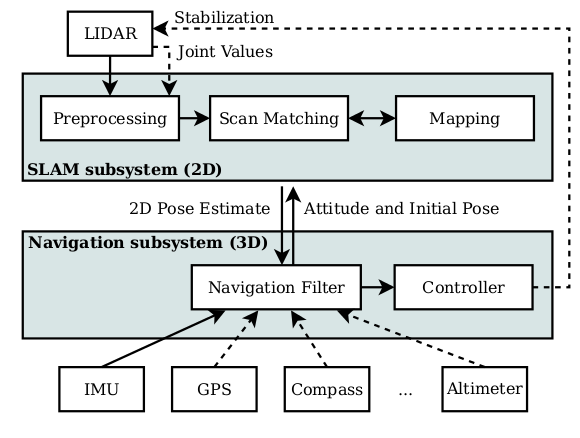
\includegraphics[width=0.5\linewidth]{hector-slam-system.png}
\end{figure}
\begin{itemize}\tiny 
\item Kohlbrecher S, Von Stryk O, Meyer J, et al. A flexible and scalable slam system with full 3d motion estimation[C]//Safety, Security, and Rescue Robotics (SSRR), 2011 IEEE International Symposium on. IEEE, 2011: 155-160.
\end{itemize}
\end{frame}

\begin{frame}{Hector SLAM}
3D state 
\begin{equation*}
\mathbf{x}=\begin{bmatrix}
\Omega^T & \mathbf{p}^T & \mathbf{v}^T
\end{bmatrix}  
\end{equation*}
where 
\begin{equation*}
\begin{split}
\Omega=\begin{bmatrix}
\phi,\theta,\varphi
\end{bmatrix} &\quad
\text{roll, pitch and yaw Euler angles}\\
\mathbf{p}=\begin{bmatrix}
\mathbf{p}_x,\mathbf{p}_y,\mathbf{p}_z
\end{bmatrix} &\quad
\text{posotion}\\
\mathbf{v}=\begin{bmatrix}
\mathbf{v}_x,\mathbf{v}_y,\mathbf{v}_z
\end{bmatrix} &\quad
\text{velocity}
\end{split}
\end{equation*} 
\begin{itemize}\tiny 
\item Kohlbrecher S, Von Stryk O, Meyer J, et al. A flexible and scalable slam system with full 3d motion estimation[C]//Safety, Security, and Rescue Robotics (SSRR), 2011 IEEE International Symposium on. IEEE, 2011: 155-160.
\end{itemize}
\end{frame}


\begin{frame}{Hector SLAM}
\begin{block}{Dynamic system}\small
\begin{equation*}
\begin{split}
\dot{\Omega}&=\mathbf{E}_\omega\cdot\omega\\
\dot{\mathbf{p}}&=\mathbf{v}\\
\dot{\mathbf{v}}&=\mathbf{R}_\omega\cdot\mathbf{a}+\mathbf{g}
\end{split}
\end{equation*} 
where\scriptsize
\begin{equation*}
\begin{split}
\mathbf{R}_\omega \quad & \text{Rotation matrix from Sensor to world}\\
\mathbf{E}_\omega \quad & \text{maps angular rates to the derivatives of the Euler angles}\\
\mathbf{g} \quad & \text{constant gravity vector}
\end{split}
\end{equation*} 
\begin{itemize}\tiny 
\item Kohlbrecher S, Von Stryk O, Meyer J, et al. A flexible and scalable slam system with full 3d motion estimation[C]//Safety, Security, and Rescue Robotics (SSRR), 2011 IEEE International Symposium on. IEEE, 2011: 155-160.
\end{itemize}
\end{block}

\end{frame}

\begin{frame}
\frametitle{Hector SLAM}
\begin{figure}
\centering
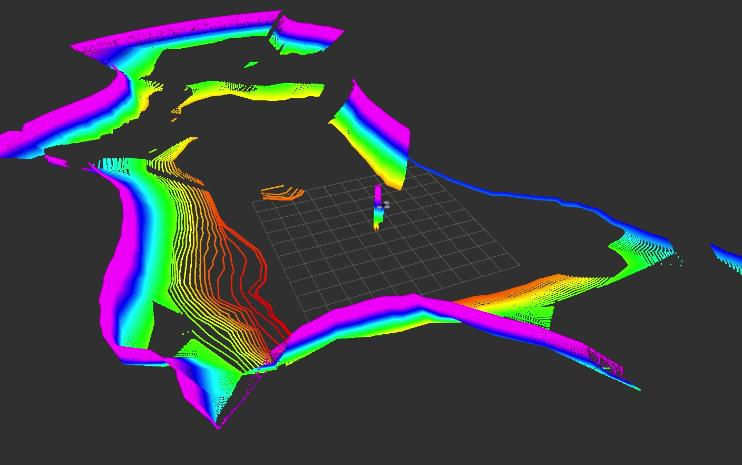
\includegraphics[width=0.6\linewidth]{hector-slam.jpg}
\end{figure}
\begin{itemize}\tiny 
\item Kohlbrecher S, Von Stryk O, Meyer J, et al. A flexible and scalable slam system with full 3d motion estimation[C]//Safety, Security, and Rescue Robotics (SSRR), 2011 IEEE International Symposium on. IEEE, 2011: 155-160.
\end{itemize}
\end{frame}
\subsection{Inertial Navigation}
\begin{frame}{Multi-Sensor Fusion}
\begin{figure}
\centering
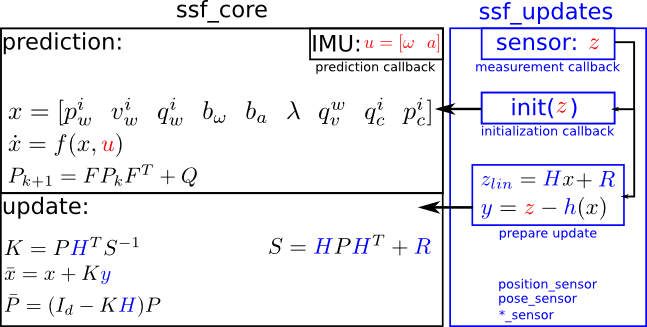
\includegraphics[width=0.5\linewidth]{msf-structure.png}
\\\quad\\
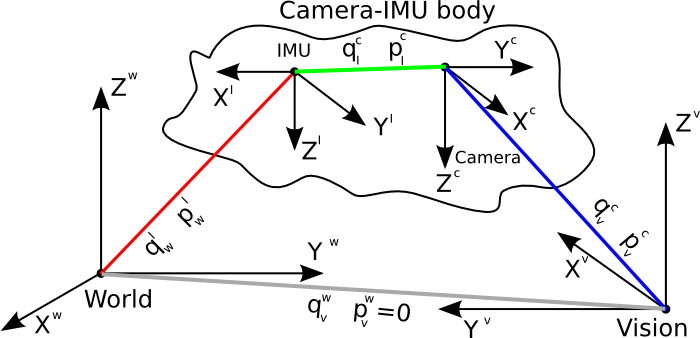
\includegraphics[width=0.5\linewidth]{framesetup.png}
\end{figure}
\begin{itemize}\tiny
\item Stephan Weiss, Markus W. Achtelik, Margarita Chli and Roland Siegwart. Versatile Distributed Pose Estimation and Sensor Self-Calibration for Autonomous MAVs. in IEEE International Conference on Robotics and Automation (ICRA), 2012. pdf
\item Stephan Weiss, Davide Scaramuzza and Roland Siegwart, Monocular-SLAM–based navigation for autonomous micro helicopters in GPS-denied environments, Journal of Field Robotics (JFR), Vol. 28, No. 6, 2011, 854-874. pdf
\end{itemize}
\end{frame}

\begin{frame}{Multi-Sensor Fusion}
\begin{figure}
\centering
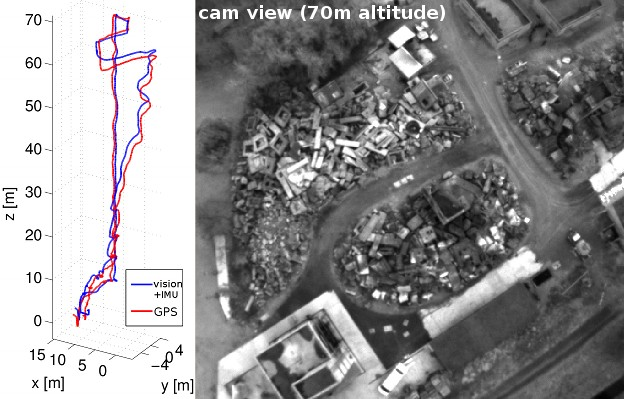
\includegraphics[width=0.5\linewidth]{ethzasl_ptam_icarus.jpg}
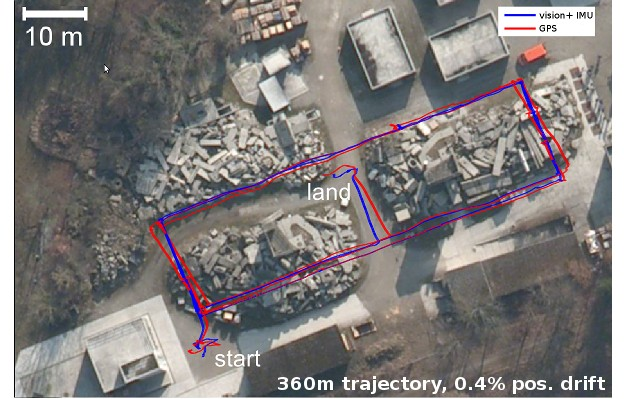
\includegraphics[width=0.5\linewidth]{ethzasl_ptam_traj.jpg}
\end{figure}
\begin{itemize}\tiny
\item Stephan Weiss, Markus W. Achtelik, Margarita Chli and Roland Siegwart. Versatile Distributed Pose Estimation and Sensor Self-Calibration for Autonomous MAVs. in IEEE International Conference on Robotics and Automation (ICRA), 2012. pdf
\item Simon Lynen, Markus Achtelik, Stephan Weiss, Margarita Chli and Roland Siegwart, A Robust and Modular Multi-Sensor Fusion Approach Applied to MAV Navigation. in Proc. of the IEEE/RSJ Conference on Intelligent Robots and Systems (IROS), 2013.
\end{itemize}
\end{frame}



\subsection{Tracking}

\begin{frame}
\frametitle{Tracking}\small
%\begin{block}{Kalman}
%\end{block}
\begin{figure}
\centering
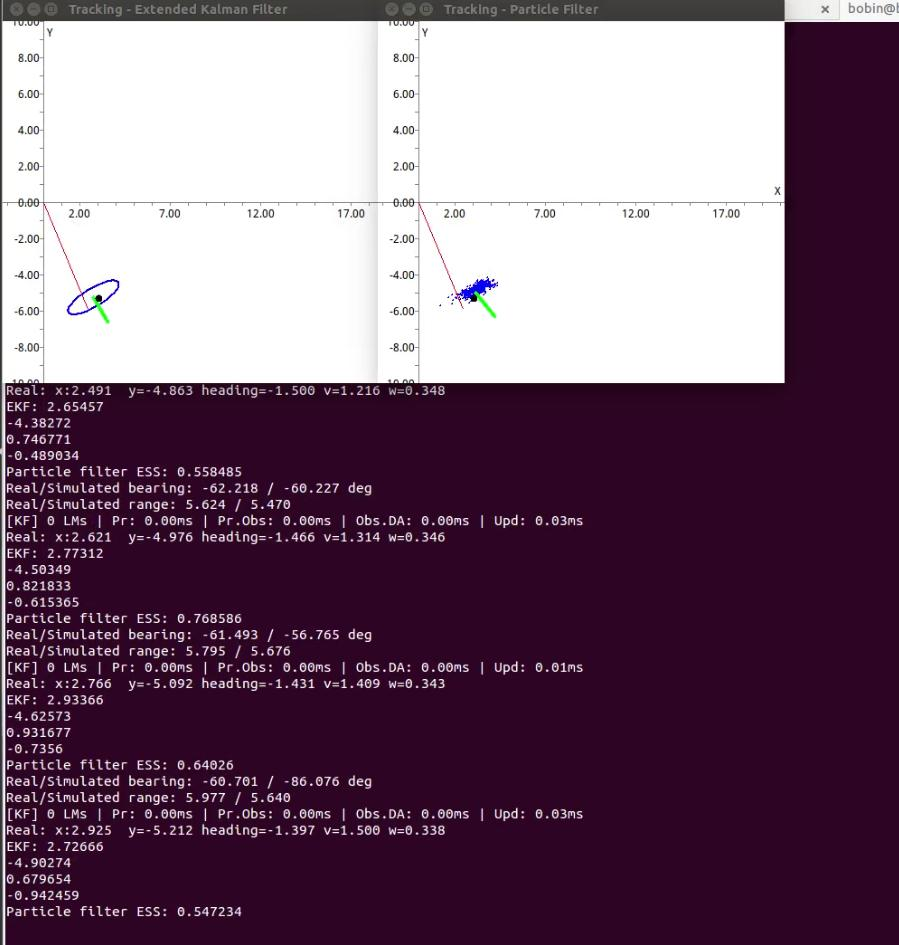
\includegraphics[width=0.5\linewidth]{tracking.jpg}
\end{figure}

\end{frame}

%\section{Conclusion}
%
%
%\begin{frame}{Reference}{}
%{\scriptsize
%\bibliographystyle{IEEEtran}
%\bibliography{IEEEabrv,ref}
%}
%\end{frame}
%
%
%\section{}


\begin{frame}
%\frametitle{Thank you}
\Huge
\begin{center}
Thank you
\end{center}
\end{frame}


\end{document}

%\begin{block}{Collaborators}
%De Xu, Zhengtao Zhang and Dapeng Zhang
%\end{block}
%\begin{block}{Foundation}
% National Nature Science Foundation under Grant 61473293, 61227804 and 61303177
%\end{block}
%\begin{block}{For more information about the research itself:}
%De Xu, Zhengtao Zhang and Dapeng Zhang
%Institute of Automation, Chinese Academy of Sciences, Beijing 100190
%E-mail: dingwendong2013@ia.ac.cn
%\end{block}

